\section{Critical Core Radius}

Neutronic viability is an important part of reactor design. The figure of merit
for neutronics is EOL \keff. The reactor must be able to sustain a fission
chain reaction from startup to shutdown on the final day of the 10 year mission.

The criticality requirement is the second of two major criteria for a valid reactor design and an
important constraint in the thermal hydraulic modeling process. As a result,
modeling criticality of various reactor configurations demands its own chapter
in this thesis. Criticality modeling started with depletion modeling, reported
in section \ref{neutronics_sweeps}. The purpose and conclusion of the depletion
modeling was that thermal power and small geometric features were of low
importance when predicting EOL \keff. In addition, higher enrichment will always
be prefferred to lower enriched uranium.

The thermal-hydraulic modeling scheme
reported in section \ref{reactor_mass_model} requires a constraint for the core
radius. A relationship between core radius and fuel fraction for a target
value of \keff was developed using traditional reactor physics tools. In lieu of
full depletion modeling, BOL \keff was modeled and the \keff target adjusted to
ensure sufficient excess reactivity for 10 years of full-power operation.

There were three major components to developing the critical core radius
constraints, determining a value for BOL excess reactivity that would satisfy
EOL \keff > 1, generating the relationship between fuel fraction and the
required core radius to meet the target \keff value. For each fuel fraction, an
optimized reflector thickness was also calculated to minimize total core mass.
It is worth noting that critical core radius is a
bit of a misnomer, since the target of this analysis was a BOL excess
reactivity.

\subsection{Critical Radius}
In order to constrain the reactor mass model, a critical radius relationship to
fuel fraction was developed. This section discusses the methods used to derive a
relationship between critical core radius and fuel fraction that was used by the
reactor mass model. 

\subsubsection{Modeling Methods}
A critical core radius curve was generated as a function of fuel fraction for
each reactor configuration. Homogeneous reactor models with optimized reflectors
were modeled with MCNP6.1. For each fuel fraction, an optimized reflector
thickness was calculated prior to the critical radius calculation. This
optimization process will be discussed in the next section.

The critical radius search process was a polynomial curve fit to MCNP-generated
\keff data. For a fixed fuel fraction, an optimized reflector thickness was
calculated. With a fuel fraction and reflector thickness fixed, \keff response
to core radius was modeled. Five kcode calculations were perfomred to generate
the \keff response to core radius. The range of core radii was determined by some
bounding calculations to be 5 to 28.75 cm. This range is a rough estimate and
could be narrowed to improve the effectiveness of the data fitting. Each radius
search started with the midpoint value of the domain. The next four data points
were spread over the first or second half of the domain depending on whether the
mid point result was greater or less than the target \keff value. The five \keff
values were reduced by the target \keff. This reduced array of values was fitted
to a second degree polynomial. The roots of the polynomial were calculated using
the NumPy function 'roots' \citep{numpy}. Roots returns all roots of any
nth-degree polynomial. The critical radius was taken to be the minimum of the
real, positive roots to the second-degree polynomial.

The critical radius search was performed for fuel fractions ranging from 0.1 to
0.9. Scipy was used to fit a power curve to the data. The resulting functions
constrain the core radius as a function of fuel fraction to the appropriate size
resulting in the desired BOL excess reactivity. Figure
\ref{fig:crit_core_radius} shows the results of the critical radius searches.

\begin{figure}[h]
    \centering
    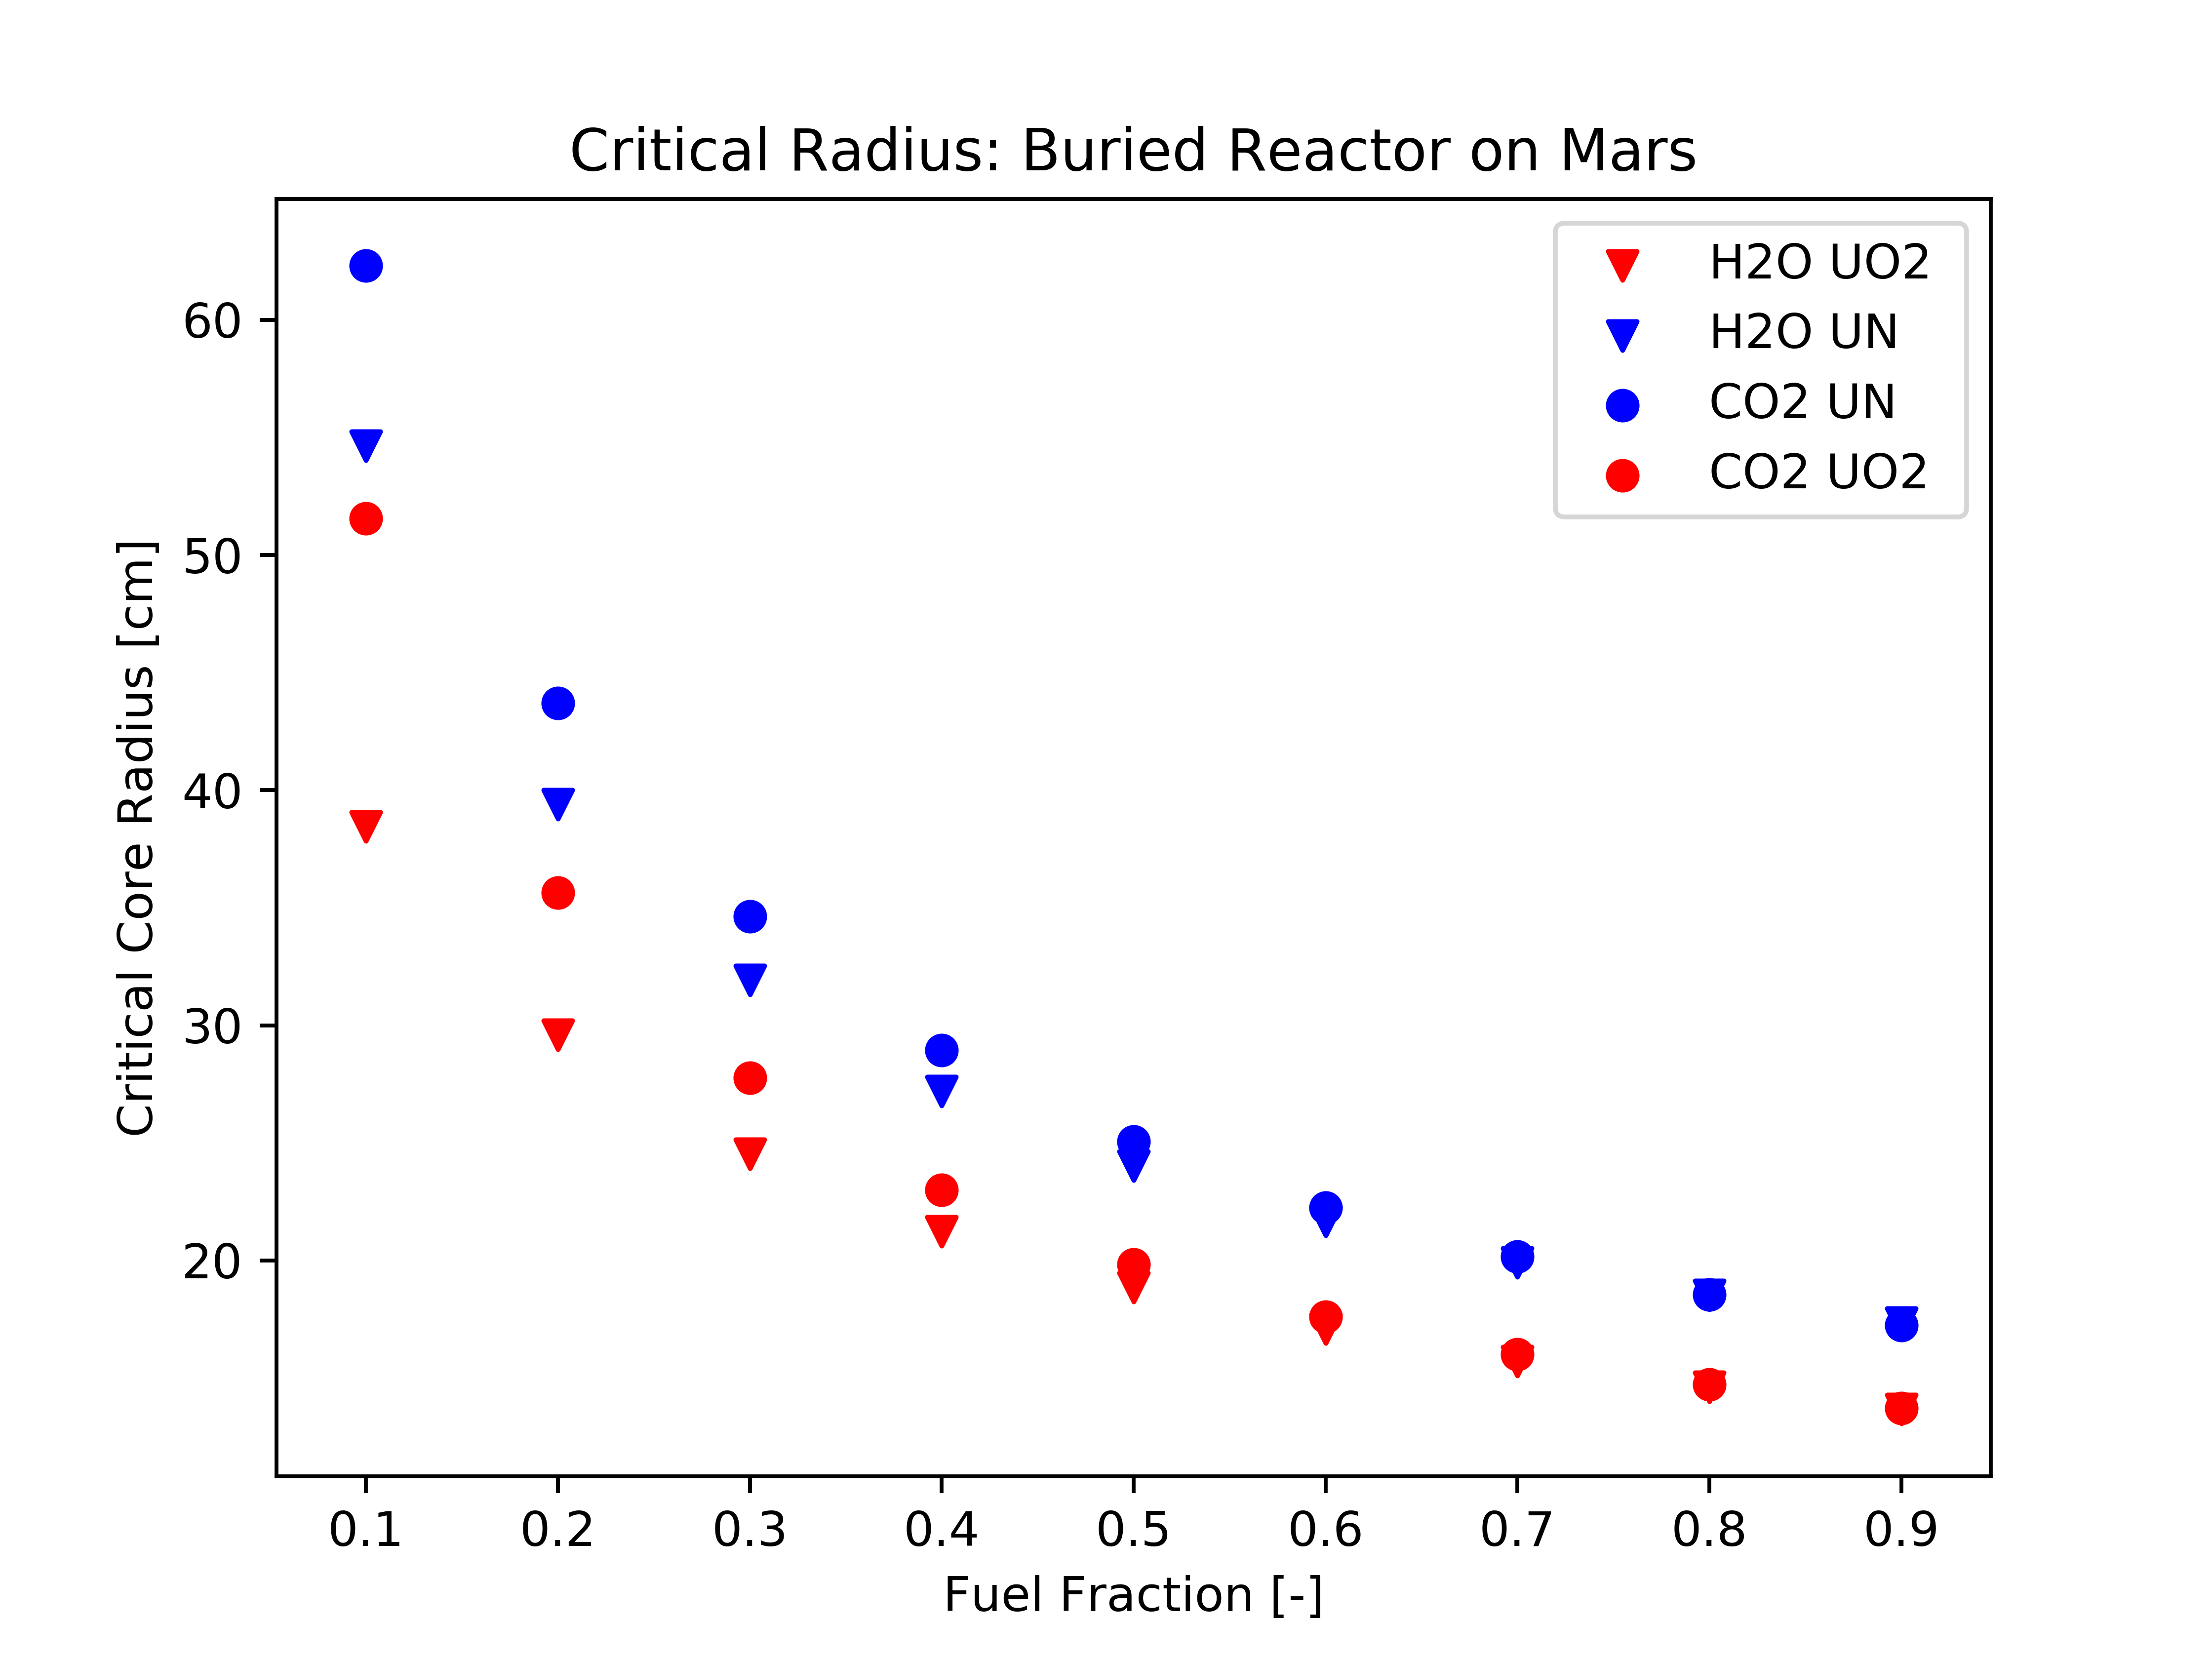
\includegraphics[width=3in]{../images/crit_radius.png}
\caption{Critical core radius results}
\label{fig:crit_core_radius}
\end{figure}

As shown in figure \ref{fig:crit_core_radius}, the \uox fuel outperforms the UW
cermet fuel in terms of critical mass. This is a result of the higher uranium
density in the \uox. The coolants impact critical radius as well, albeit to a
lesser extent. The \water
provides some moderation that helps improve the fission cross section in the
fuel. As the fuel fraction approaches 1, the difference in coolant is
negligible. These results were fit to a power function, shown in Equation
\ref{eq:power_fit}.

\begin{equation}
    R_{core} = A*exp(-B*frac_{fuel})
    \label{eq:power_fit}
\end{equation}

The resulting coefficients for each reactor configuration are shown below in
Table \ref{tab:crit_radius_coeffs}.

\begin{table}[h]
  \centering
  \caption{Critical Radius Fits}
  \begin{tabular}{ccc}
    \toprule
    Reactor Configuration   &   A [cm]  &  B [-]   \\
    \midrule 
     \uox-\codiox	        & 13.224     &  -0.596 \\
     \uox-\water            & 13.674     &  -0.458 \\
     UW-\codiox             & 16.871     &  -0.573 \\
     UW-\water              & 16.817     &  -0.516 \\
  \end{tabular}
  \label{tab:crit_radius_coeffs}
\end{table}

\subsection{Optimized Reflector Thicknesses}
Reflectors are used in nuclear reactor design to reduce neutron leakage from the
reactor core. Reflectors can reduce required fuel mass by reflecting neutrons
back into the core and preventing them from being lost to leakage. However,
adding reflector thickness to the outside of the core adds mass to the overall
reactor system. There is a tradeoff between mass of fuel and mass of
reflector and an optimal combination of the two. The purpose of this analysis
was to optimize reflector thickness as a multiplier of the overall core radius.
This analysis was done for each fuel-coolant combination.

\subsubsection{Modeling Methods}
Reflector thickness was defined as a multiplier of core radius. Each reactor
fuel-coolant combination was modeled with various reflector thickness
multipliers. Homogeneous reactor core models with reflectors were modeled with
MCNP6.1. A range of reflector multipliers was explored to determine the optimum
multiplier that minimzed overall core mass. For each reflector multiplier, a critical radius search was performed
to reach the target criticality found in section \ref{neutronics_sweeps}. Each
critical core with its reflector has a corresponding total mass. A 3rd degree
polynomial curve was fit to the mass results with SciPy\citep{scipy}. The global
minima of this curve was found unsing Scipy's optimization capabilities to
minimize the mass response. The
reflector multiplier that minimized the total core mass was chosen as the
optimized reflector for each fuel fraction.
This was done for each reactor fuel-coolant combination and a set of optimal
reflector multiplier values was created.

Figure REF THE FIGURES HERE, shows the reactor mass results as a function of
reflector multiplier for a fixed fuel fraction. For small multipliers, increasing the reflector thickness
lowers the required fuel mass and as a result, the overall reactor mass. As the
reflector thickness continues to grow, there are diminishing returns. Adding
more reflector mass does not reduce fuel mass and the total reactor mass starts
to grow again. Table \ref{tab:ref_mult} shows the optimized reflector
thicknesses.

\begin{figure}[h]
    \centering
    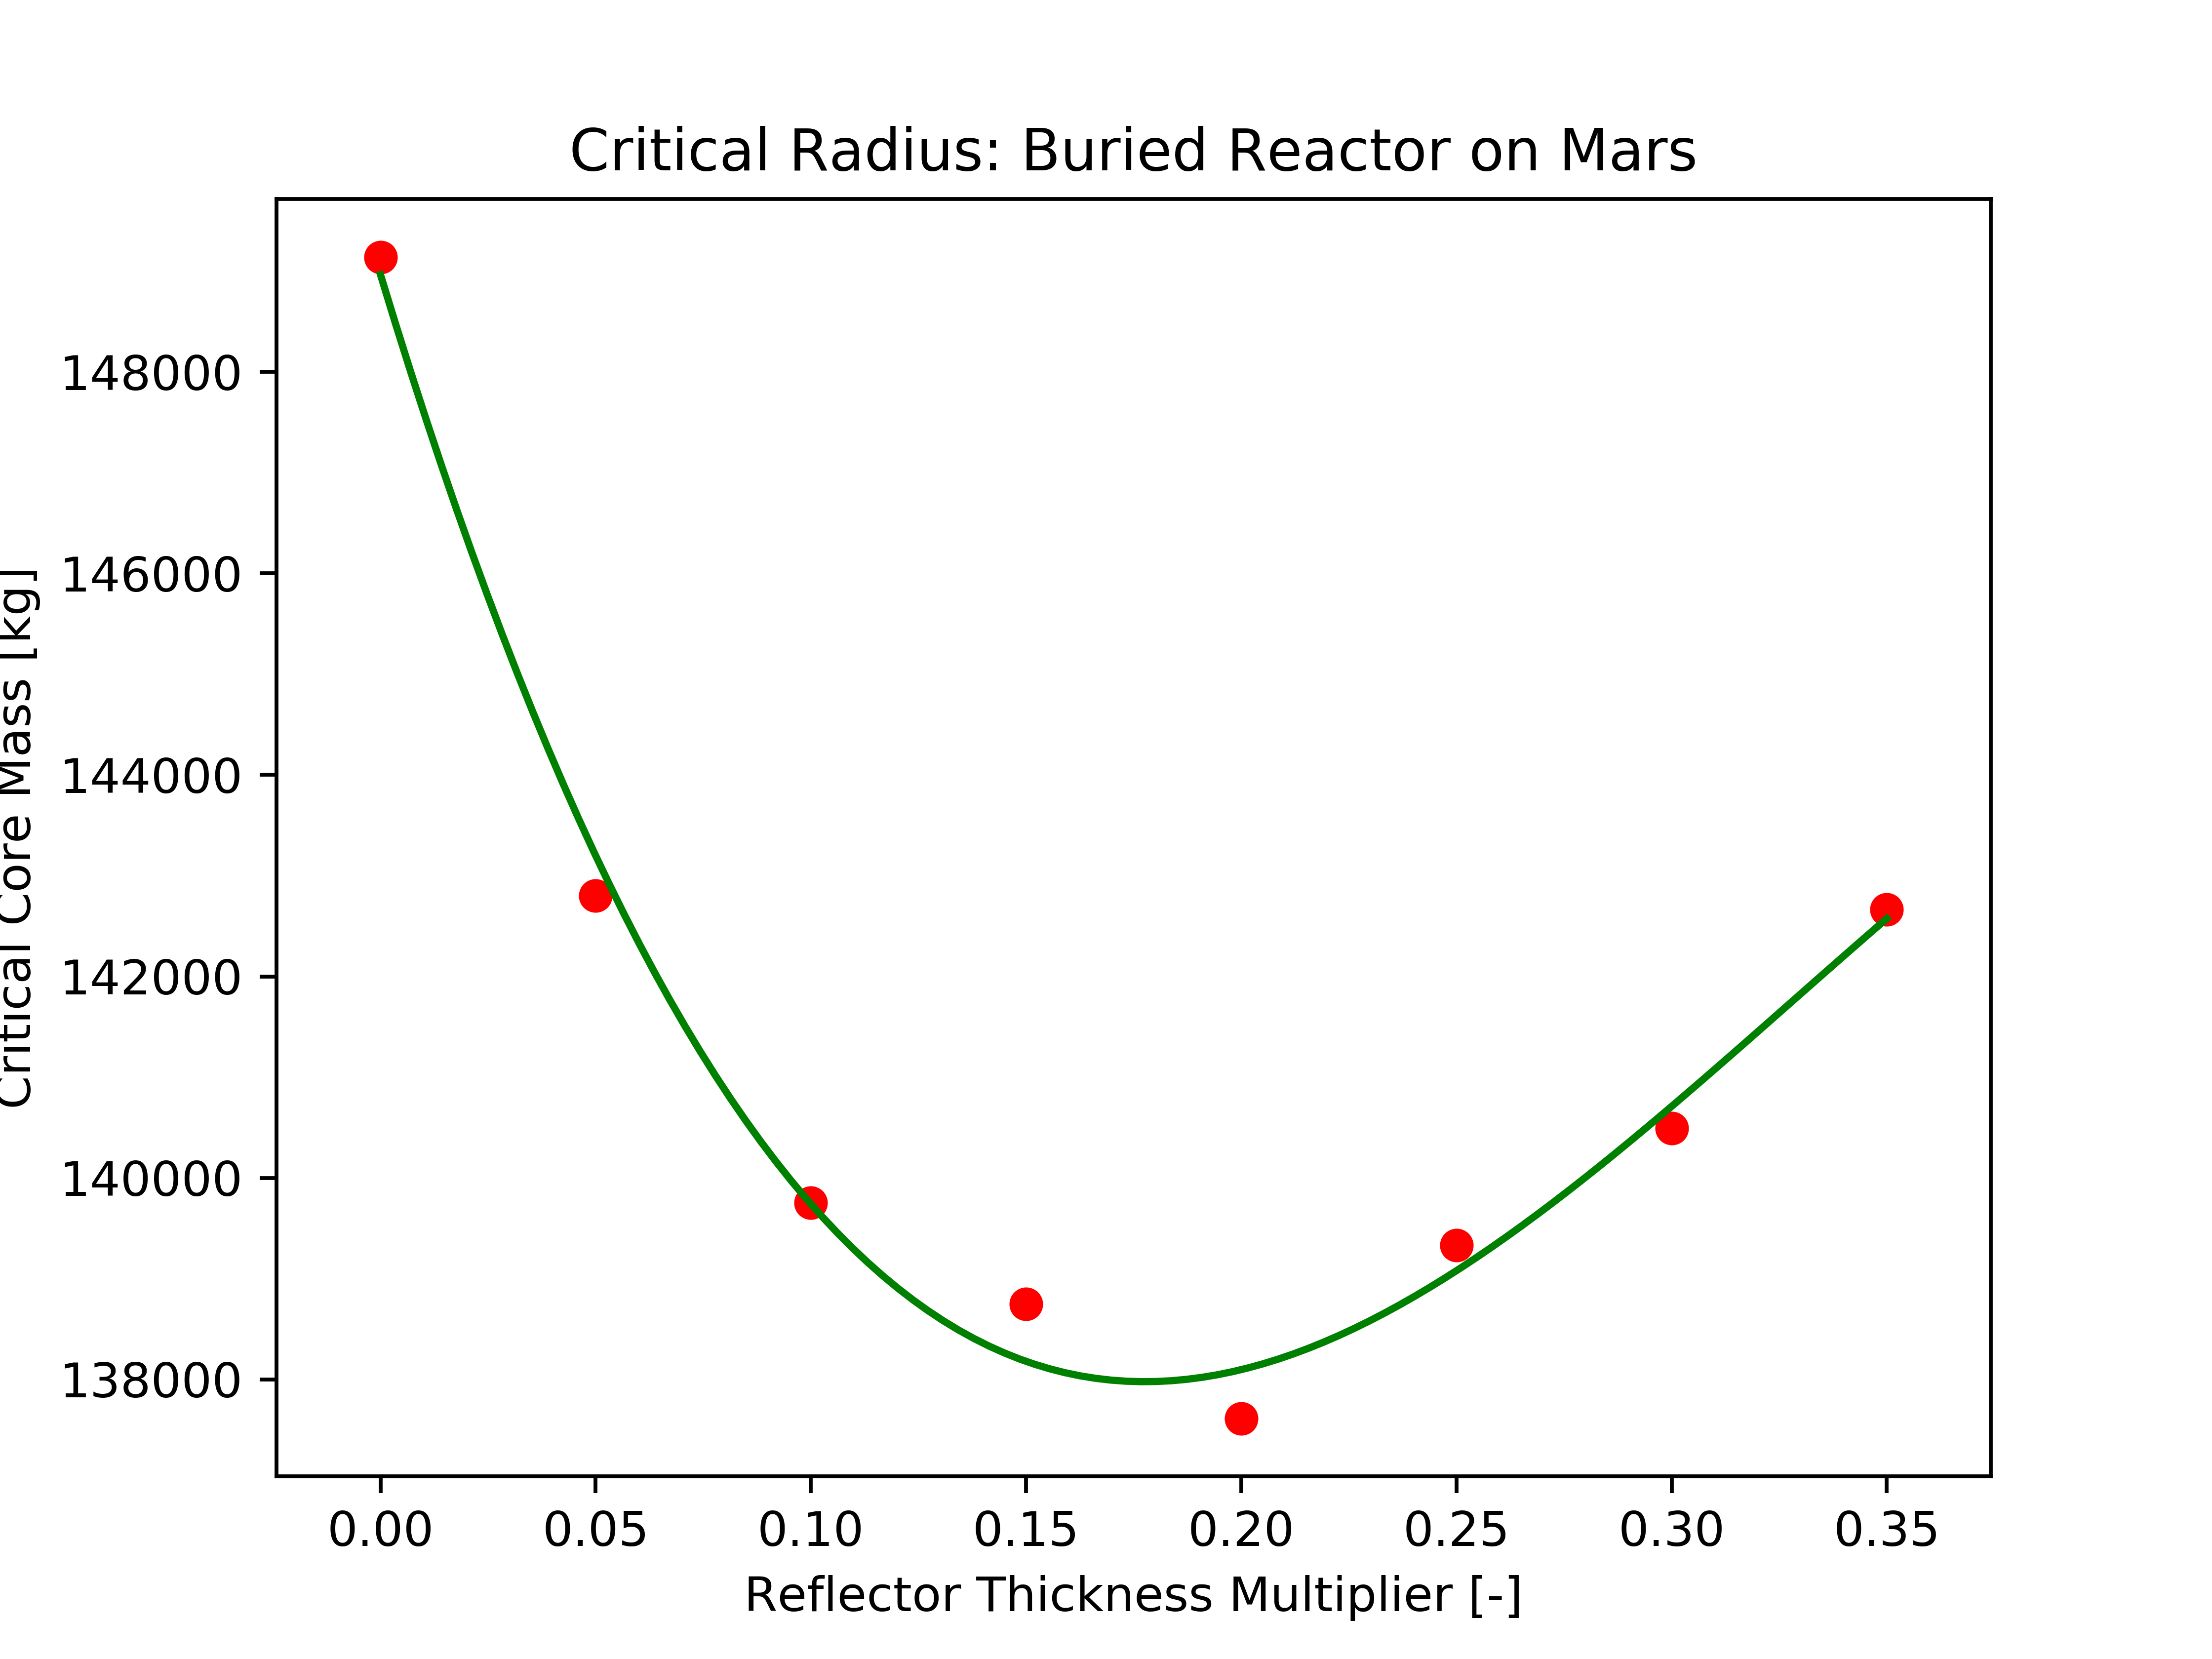
\includegraphics[width=3in]{../images/opt_refl_CO2_UO2.png}
\caption{\codiox \uox optimal reflector thickness}
\label{fig:uo2_co2_refl}
\end{figure}

\begin{figure}[h]
    \centering
    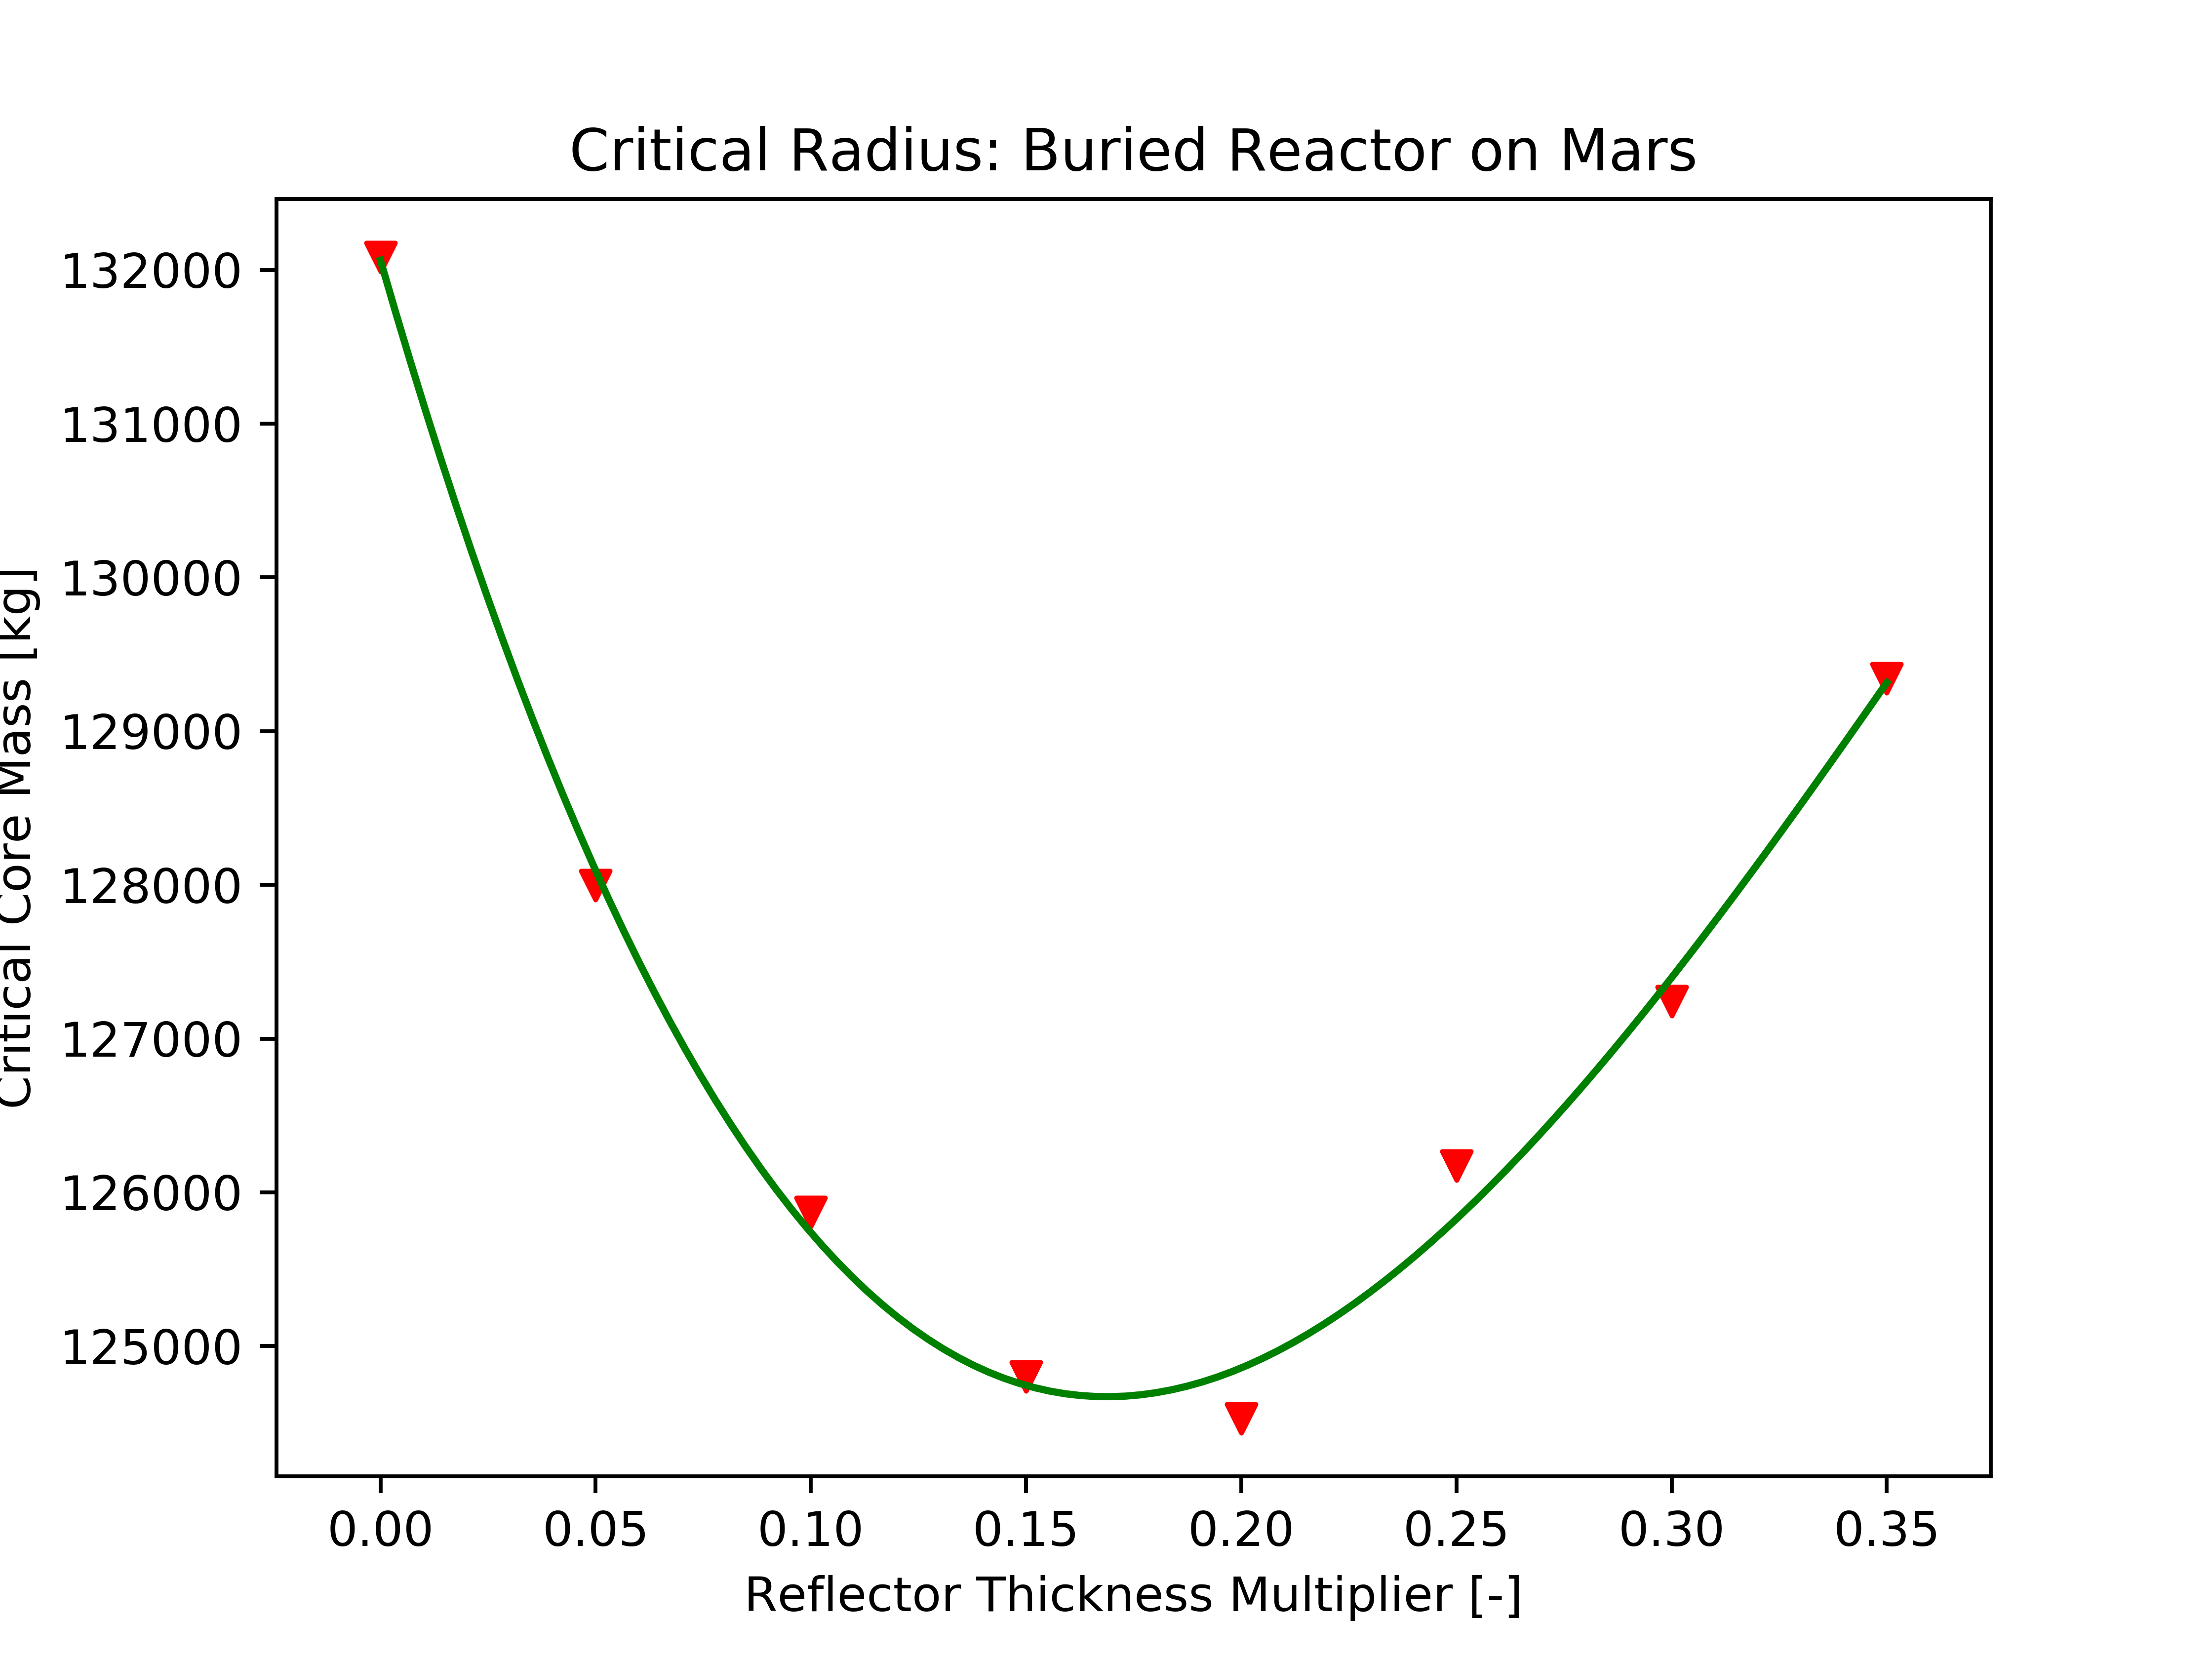
\includegraphics[width=3in]{../images/opt_refl_H2O_UO2.png}
\caption{\water \uox optimal reflector thickness}
\label{fig:uo2_h2o_refl}
\end{figure}

\begin{figure}[h]
    \centering
    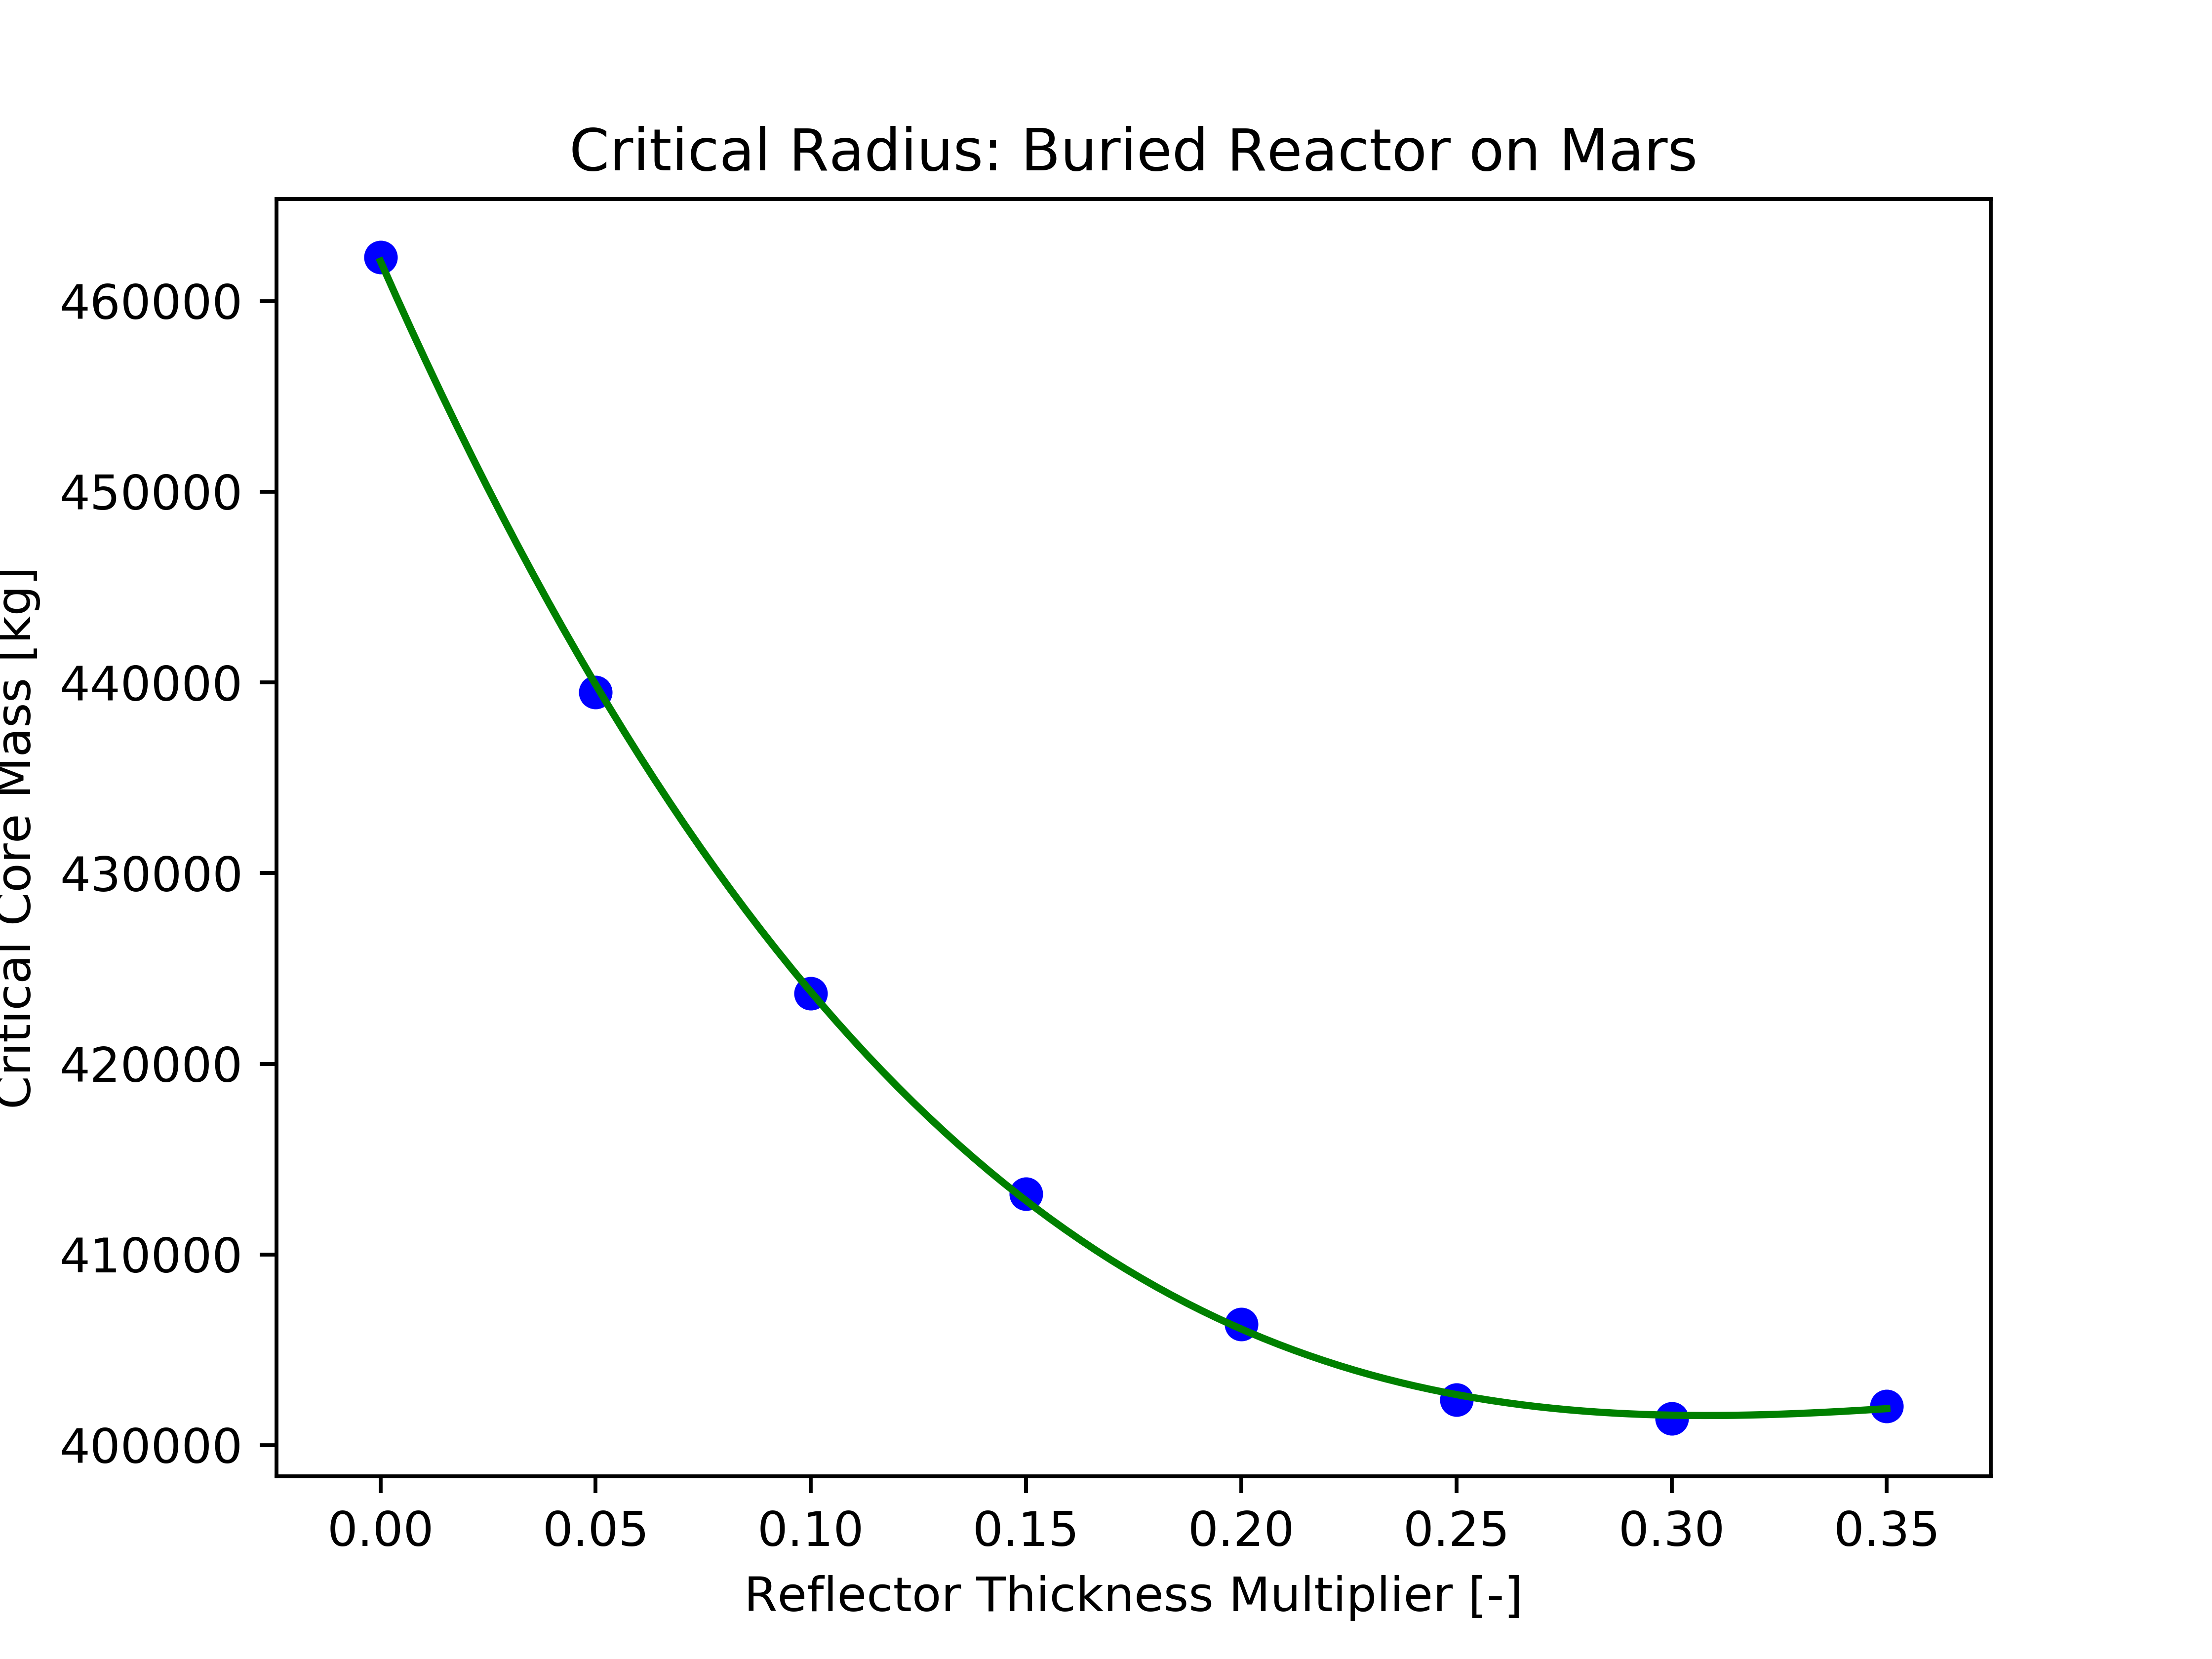
\includegraphics[width=3in]{../images/opt_refl_CO2_UN.png}
\caption{\codiox UW optimal reflector thickness}
\label{fig:uw_co2_refl}
\end{figure}

\begin{figure}[h]
    \centering
    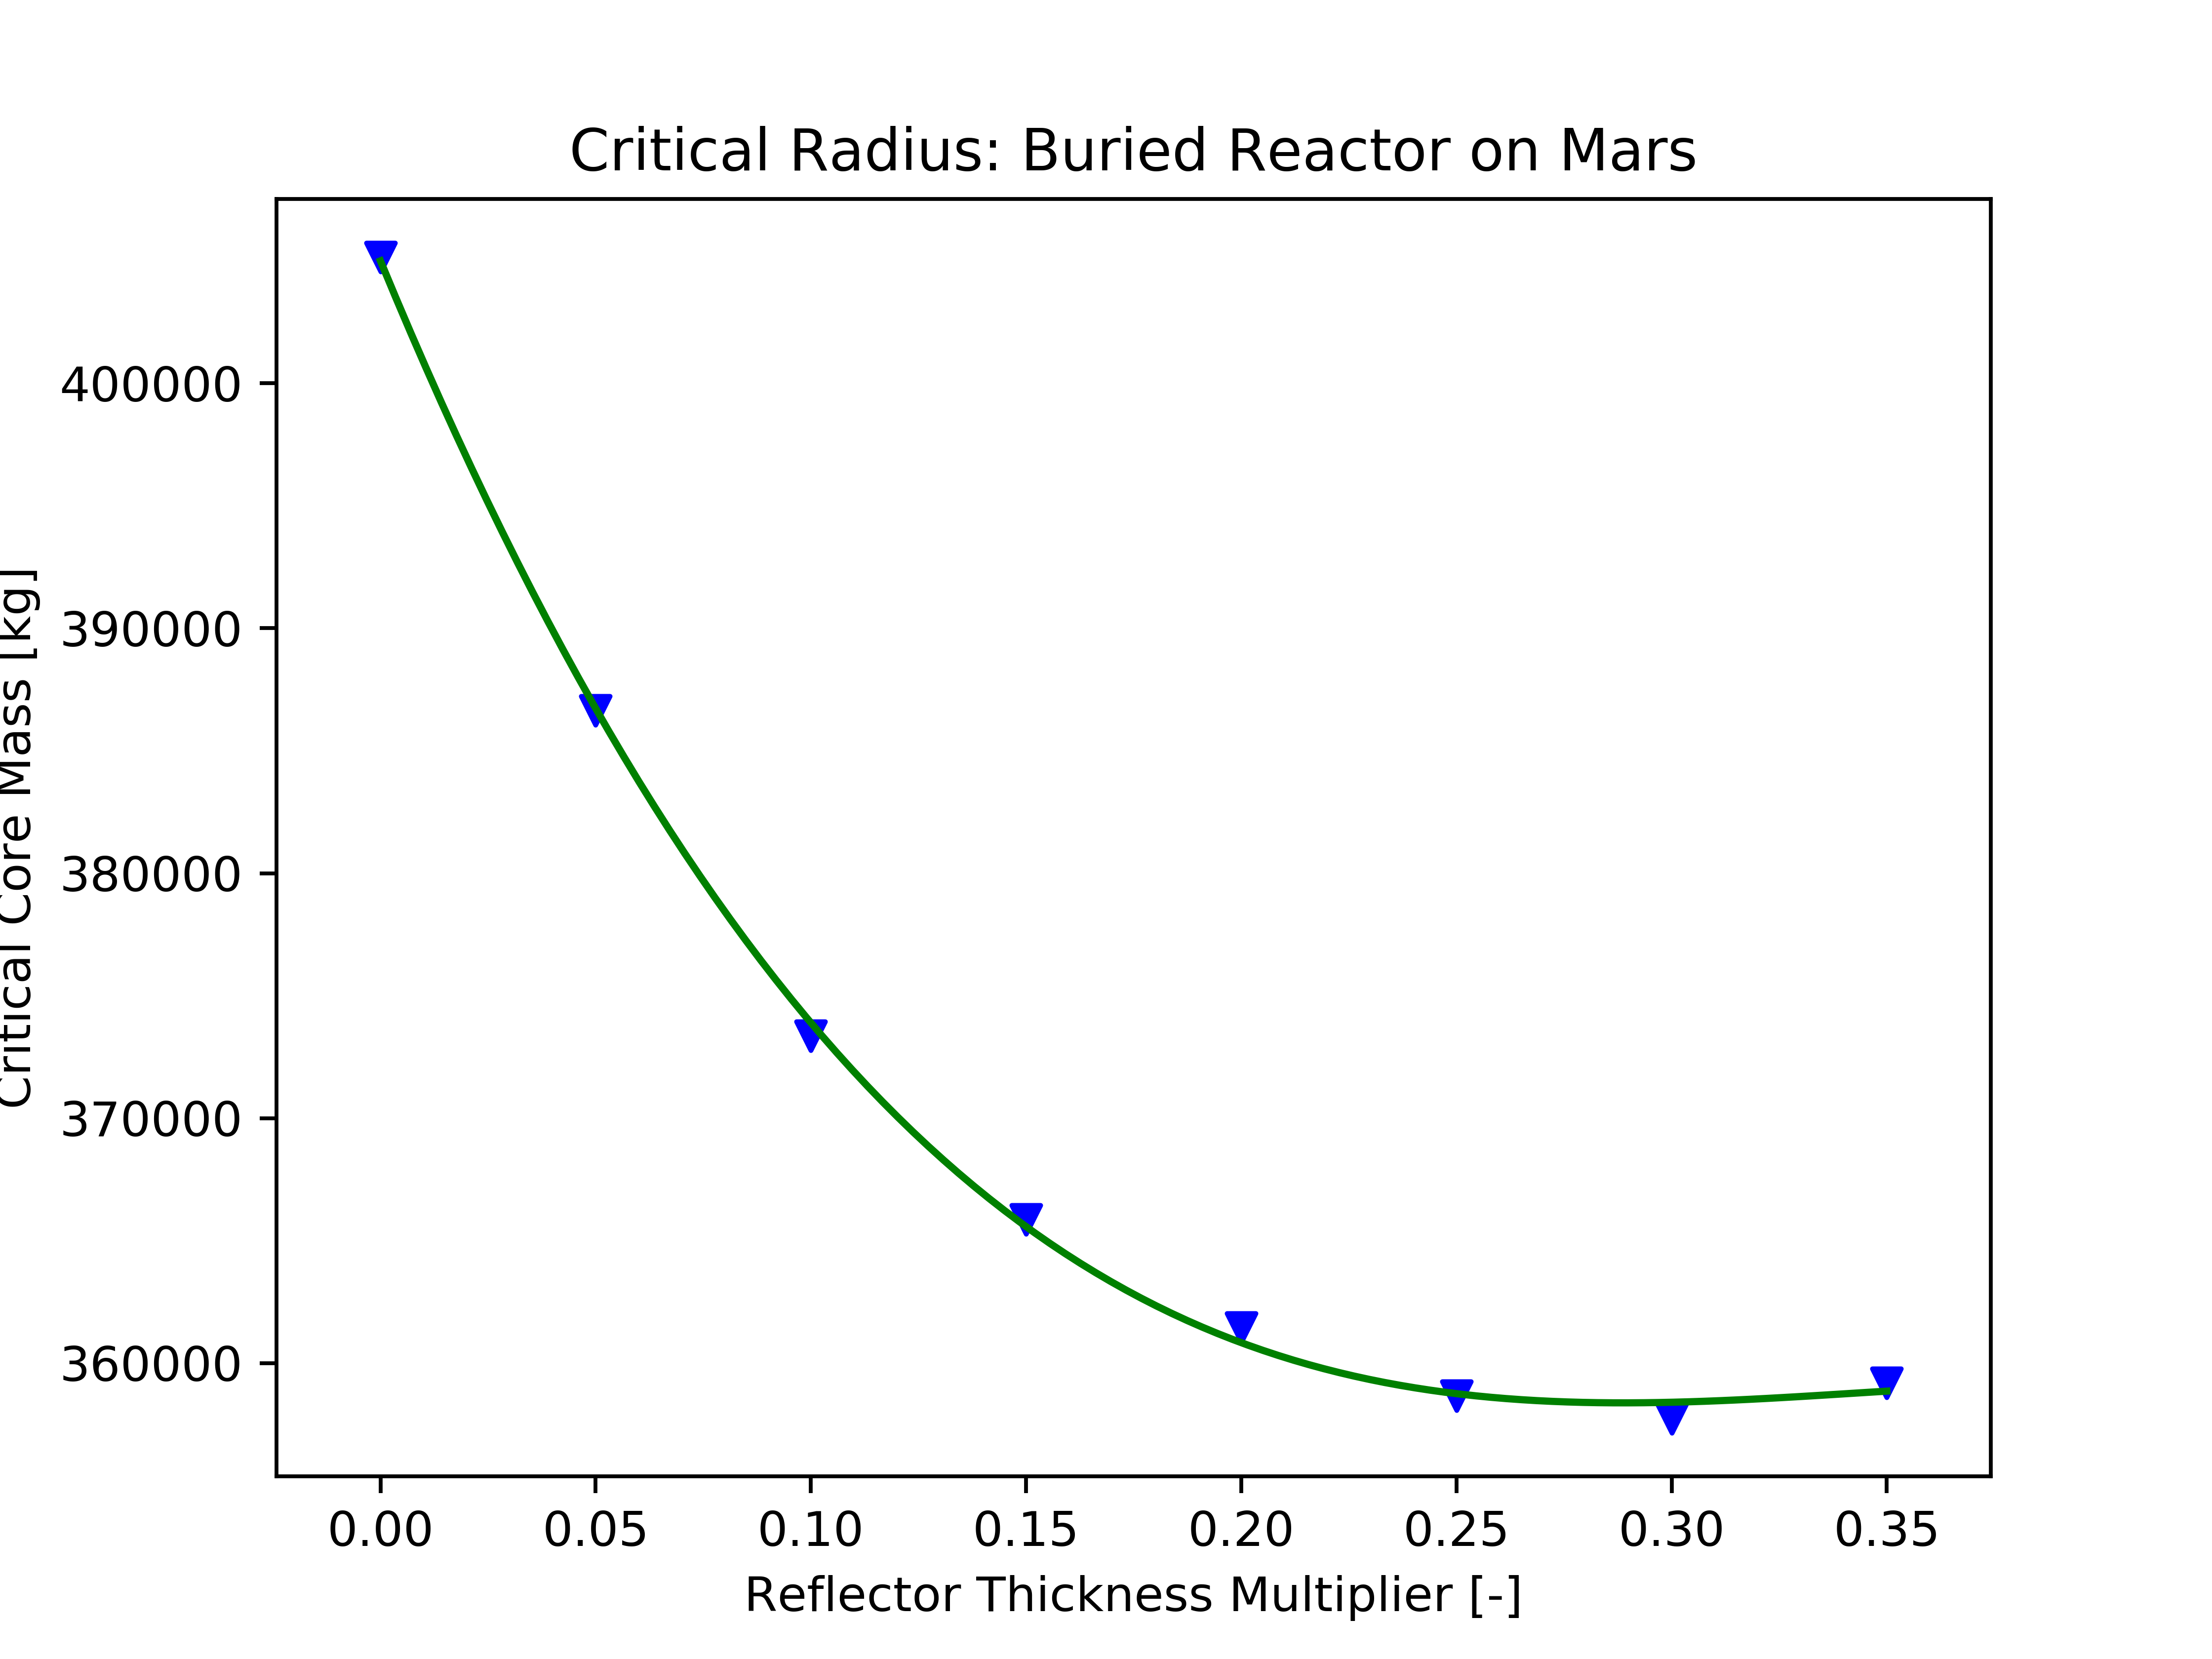
\includegraphics[width=3in]{../images/opt_refl_H2O_UN.png}
\caption{\water \uox optimal reflector thickness}
\label{fig:uw_h2o_refl}
\end{figure}

\begin{table}[h]
  \centering
  \caption{Optimized Reflector Thickness Multipliers}
  \begin{tabular}{cc}
    \toprule
    Reactor Configuration   & Reflector Multiplier [-] \\
    \midrule 
     \uox-\codiox	        & 1.165 \\
     \uox-\water            & 1.158 \\
     UW-\codiox             & 1.344 \\
     UW-\water              & 1.296 \\
  \end{tabular}
  \label{tab:ref_mult}
\end{table}

These figures demonstrate the process to select an optimal reflector thickness.
Each fuel fraction has a unique optimal reflector multiplier. This optimization
was performed for each fuel fraction as part of the critical radius searches.
Figures REF TEH FIGURES HERE show the result for
each core of the reflector optimization as a function of fuel fraction.

